\documentclass{article}
\usepackage[letterpaper,top=2cm,bottom=2cm,left=3cm,right=3cm,marginparwidth=1.75cm]{geometry}
\usepackage{amsmath}
\usepackage{amssymb}
\usepackage{tikz}
\usepackage{pgfplots}

\newcommand{\solution}{\textbf{Solution: }}
\newcommand{\der}[3][]{\frac{d^{#1} #2}{d #3^{#1}}}
\newcommand{\pder}[3][]{\frac{\partial^{#1} #2}{\partial #3^{#1}}}
\newcommand{\inv}{^{-1}}

\pgfplotsset{compat = newest}
\setlength\parindent{0pt}

\title{Math 20D HW3}
\author{Merrick Qiu}


\begin{document}
\maketitle

\subsection*{Section4.3}
\textbf{Problem 3}
The roots are 
\[
    r^2- 6r + 10 
    \implies r = \frac{6 \pm \sqrt{36-40}}{2}
    \implies r = 3 \pm i
\]
The general solution is
\[
    y = c_1e^{3t}\cos t + c_2e^{3t}\sin t
\]
\textbf{Problem 6}
The roots are 
\[
    r^2-4r+7
    \implies r = \frac{4 \pm \sqrt{16-28}}{2}
    \implies r = 2 \pm \sqrt{3}i
\]
The general solution is 
\[
    y = c_1e^{2t}\cos (\sqrt{3}t) + c_2e^{2t}\sin (\sqrt{3}t)
\]
\textbf{Problem 17}
The roots are 
\[
    r^2-r+7 = 0 
    \implies r = \frac{1 \pm \sqrt{1-28}}{2}
    \implies r = \frac{1}{2} \pm \frac{3\sqrt{3}}{2}
\]
The general solution is 
\[
    y = c_1e^{\frac{t}{2}}\cos (\frac{3\sqrt{3}t}{2}) + 
        c_2e^{\frac{t}{2}}\sin (\frac{3\sqrt{3}t}{2})
\]
\textbf{Problem 24}
The roots are 
\[
    r^2 + 9 = 0
    \implies r = 3i
\]
The general solution is 
\[
    y = c_1\cos 3t + c_2\sin 3t
\]
At the initial conditions,
\[
    1 = c_1
\]
\[
    1 = 3c_2
\]
The final solution is 
\[
    y = \cos 3t + \frac{1}{3}\sin 3t
\]
\textbf{Problem 25}
The roots are 
\[
    r^2 - 2r + 2 = 0
    \implies r = \frac{2 \pm \sqrt{4-8}}{2}
    \implies r = 1 \pm i
\]
The general solution is 
\[
    y = c_1e^t\cos t + c_2e^t\sin t
\]
At the initial conditions,
\[
    e^\pi = -c_1e^\pi 
\]
\[
    0 = c_1e^\pi-c_2e^\pi
\]
The final solution is 
\[
    y = e^t\sin t - e^t\cos t
\]
\textbf{Problem 26}
The roots are 
\[
    r^2 - 2r + 1 = 0
    \implies r = \frac{2 \pm \sqrt{4-4}}{2}
    \implies r = 1
\]
The general solution is 
\[
    y = c_1e^t + c_2te^t
\]
At the initial conditions,
\[
    1 = c_1 
\]
\[
    -2 = c_1 + c_2
\]
The final solution is 
\[
    y = e^t - 3te^t
\]
\textbf{Problem 28}
The roots are 
\[
    r^2 + br + 4 = 0
    \implies r = \frac{-b \pm \sqrt{b^2-16}}{2}
\]
For $b=5$,
\[
    r_5 = -\frac{5}{2} \pm \frac{3}{2}
    \implies r_5 = -4, -1
\]
The general solution is 
\[
    y_5 = c_1e^{-4t} + c_2e^{-t}
\]
At the initial conditions,
\[
    1 = c_1 + c_2
\]
\[
    0 = -4c_1 - c_2
\]
The final solution is 
\[
    y_5 = -\frac{1}{3}e^{-4t} + \frac{4}{3}e^{-t}
\]
For $b=4$,
\[
    r_4 = -2
\]
The general solution is 
\[
    y_4 = c_1e^{-2t} + c_2te^{-2t}
\]
At the initial conditions,
\[
    1 = c_1 
\]
\[
    0 = -2c_1 + c_2
\]
The final solution is 
\[
    y_4 = e^{-2t} + 2te^{-2t}
\]
For $b=2$,
\[
    r_2 = -1 \pm \sqrt{3}i
\]
The general solution is 
\[
    y_2 = c_1e^{-t}\cos \sqrt{3}t + c_2e^{-t}\sin \sqrt{3}t
\]
At the initial conditions,
\[
    1 = c_1
\]
\[
    0 = -c_1 + \sqrt{3} c_2
\]
The final solution is 
\[
    y_2 = e^{-t}\cos \sqrt{3}t + \frac{1}{\sqrt{3}}e^{-t}\sin \sqrt{3}t
\]
Graphing the equations yields
(not quite sure why $b=2$ graph isn't working),

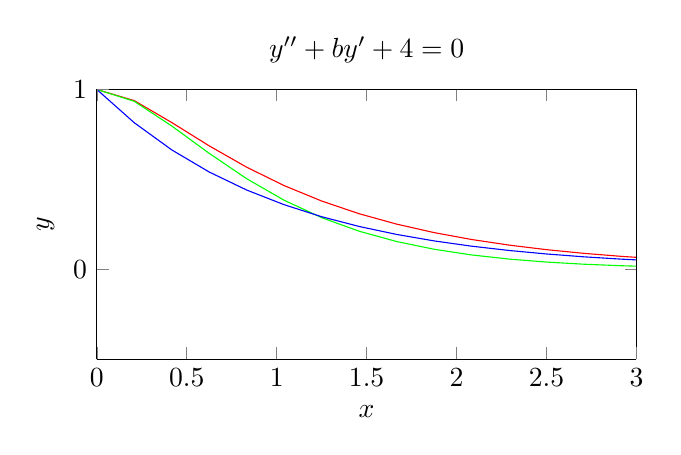
\begin{tikzpicture}
    \begin{axis}[
        xmin = 0, xmax = 3,
        ymin = -0.5, ymax = 1,
        zmin = 0, zmax = 1,
        axis equal image,
        view = {0}{90},
        title = {$y''+by'+4=0$},
        xlabel = {$x$},
        ylabel = {$y$},
    ]
    \addplot[red, domain=0:5]{-e^(-4*x)/3 + 4*e^(-x)/3};
    \addplot[green, domain=0:5]{e^(-2*x)+2*x*e^(-2*x)};
    \addplot[blue, domain=-0:5]{e^(-x)*(cos(sqrt(3)*x) + sin(sqrt(3)*x)/sqrt(3))};
    
    \end{axis}
\end{tikzpicture}

\subsection*{Section 4-4}
\textbf{Problem 4}
Method works since $3^t = e^(\ln 3 t)$

\textbf{Problem 11}
The roots are 
\[
    r^2 + r = 0 \implies r=-1, 0
\]
Since $r=\ln2$ is not a root, the general form is 
\[
    y = A_0 2^x
\]
Plugging this into the original equation yields 
\[
    \ln(2)^2 A_0 2^x + A_02^x = 2^x
    \implies A_0 = \frac{1}{\ln(2)^2+1}
\]
The particular solution is 
\[
    y = \frac{2^x}{\ln(2)^2+1}
\]

\textbf{Problem 14}
The roots are 
\[
    2r^2 + 1 = 0 \implies r = \frac{1}{\sqrt{2}}i
\]
Since $r = 2$ is not a root, the general form is 
\[
    y = A_0 e^{2t}
\]
Plugging this into the original equation yields 
\[
    8A_0e^{2t} + A_0 e^{2t} = 9e^{2t}
    \implies A_0 = 1
\]
The particular solution is 
\[
    y = e^{2t}
\]
\textbf{Problem 18}
The roots are 
\[
    r^2-2r+1 = 0
    \implies r=1
\]
Since $r=1$ is a double root, the general form is 
\[
    y = A_0 t^2e^t
\]
Plugging this into the original equation yields 
\[
    A_0((2e^t+ 2te^t + 2te^t + t^2e^t) - 2(2te^t + t^2e^t) + (t^2e^t)) = 8e^t
    \implies A_0(2e^t) = 8e^t
    \implies A_0 = 4
\]
The particular solution is 
\[
    y = 4 t^2e^t
\]
\textbf{Problem 25}
The roots are 
\[
    r^2 + 2r + 4 = 0 
    \implies r = \frac{-2 \pm \sqrt{4-16}}{2}
    \implies r = -1 \pm \sqrt{3}i
\]
$2 + 3i$ is not a root, so the general solution is 
\[
    y = e^{2t}(A \cos 3t + B \sin 3t)
\]
Finding the derivatives yields
\begin{align*}
    y' 
    &= 2e^{2t}(A \cos 3t + B \sin 3t) + e^{2t}(-3A \sin 3t + 3B \cos 3t) \\
    &= e^{2t}((2A+3B)\cos 3t + (-3A+2B) \sin 3t)
\end{align*}
\begin{align*}
    y''
    &= 2e^{2t}((2A+3B)\cos 3t + (-3A+2B) \sin 3t) + e^{2t}((-6A-9B)\sin 3t + (-9A+6B) \cos 3t) \\
    &= e^{2t}((-5A+12B)\cos 3t + (-12A-5B) \sin 3t)
\end{align*}
Plugging these into the original equation yields,
\[
    (3A+18B)\cos 3t + (-18A+3B)\sin 3t = 111 \cos 3t
\]
Therefore, the particular solution is 
\[
    y = e^{2t}(\cos 3t + 6 \sin 3t)
\]
\textbf{Problem 28}
The auxillary equation has the double root $r=3$, so $s=2$.
\[
    y = t^2(A_6t^6+A_5t^5+A_4t^4+A_3t^3+A_2t^2+A_1t+A_0)e^{3t}
\]

\textbf{Problem 31}
The auxillary equation has roots $r = -1 \pm i$, so $s=1$
\[
    y = t(A_3t^3+A_2t^2+A_1t+A_0)e^{-t}\cos t + 
    t(B_3t^3+B_2t^2+B_1t+B_0)e^{-t}\sin t 
\]
\textbf{Problem 32}
The auxillary equation has roots $r=-3, 4$ so $s=1$
\[
    y = t(A_3t^3+A_2t^2+A_1t+A_0)e^{-3t}
\]
\subsection*{Section 4-5}
\textbf{Problem 1}
\begin{enumerate}
    \item $5\cos t$
    \item $\cos t - e^{2t}$
    \item $4\cos +6e^{2t}$
\end{enumerate}
\textbf{Problem 4}
The roots are 
\[
    r^2 + r = 0 \implies r = -1, 0
\]
The general solution is therefore 
\[
    y = t + C_1e^{-t} + C_2
\]
\textbf{Problem 18}
The roots are 
\[
    r^2-1 = 0 \implies r=-1, 1
\]
The particular solution has form 
\[
    y_p(t) = A_1t + A_0
\]
Solving for the coefficients yields 
\[
    y_p(t) = 11t - 1
\]
The general solution is therefore
\[
    y(t) = 11t-1 + C_1e^{-t} + C_2e^t
\]
\textbf{Problem 23}
The equation is linear and the integrating factor is 
\[
    \mu = e^{-x}
\]
Multiplying both sides by the integrating factor yields 
\[
   \der{}{x} e^{-x}y = e^{-x}
   \implies e^{-x}y = -e^{-x}
   \implies y = -1
\]
The equation has root $r=1$, so the general form is 
\[
    y = Ce^t-1
\]
At $y(0) = 0$,
\[
    y = e^t-1
\]

\textbf{Problem 24}
Integrating twice yields 
\[
    y' = 3t^2 + C_1
\]
\[
    y = t^3 + C_1t + C_2
\]
At the initial values $C_1 = -1$ and $C_2 = 3$, 
\[
    y = t^3 - t + 3
\]

\textbf{Problem 25}
The roots are 
\[
    r^2 + 1 = 0 \implies r = \pm i
\]
The homogenous solution is therefore 
\[
    y_h = C_1\cos x + C_2\sin x
\]
The particular solution is in the form 
\[
    y_p = A_0e^{-x}
\]
Solving gives $A_0 = 1$ .
The general solution has form 
\[
    y = e^{-x} + C_1\cos x + C_2\sin x
\]
Solving for constants yields 
\[
    y = e^{-x} - \cos x + \sin x
\]
\textbf{Problem 28}
The roots are 
\[
    r^2 + r - 12 = 0 
    \implies (r+4)(r-3) = 0
    \implies r=-4, r=3
\]
The homogenous solution is 
\[
    y_h = C_1e^{-4t} + C_2{3t}
\]
For $r=1,2$ are not roots, so the particular solution has form 
\[
    y_p = Ae^t + Be^{2t} + \frac{1}{12}
\]
Solving for the constants gives $A=-\frac{1}{10}$ and $B=-\frac{1}{3}$
The general solution has form 
\[
    y = -\frac{1}{10}e^t - \frac{1}{6}e^{2t} + \frac{1}{12} + C_1e^{-4t} + C_2{3t}
\]
Plugging in the initial values gives 
\[
    1 = -\frac{4}{15} + C_1 + C_2
\]
\[
    3 = -\frac{13}{30} -4C_1 + 3C_2
\]
Therefore the final solution is 
\[
    y = -\frac{1}{10}e^t - \frac{1}{6}e^{2t} + \frac{1}{12} + \frac{1}{60}e^{-4t} + \frac{7}{6}{3t}
\]


\end{document} 
